\documentclass[11pt]{article}

%\usepackage{palatino}

\usepackage[utf8]{inputenc}
\usepackage[T1]{fontenc}
% Chivo como en las diapositivas o Fira Sans?
% \usepackage[familydefault,regular]{Chivo}
%\usepackage[sfdefault,scaled=.85]{FiraSans}
%\usepackage{newtxsf}
\usepackage[spanish]{babel}
\setlength{\parindent}{0pt}
\usepackage{amssymb}
\usepackage{amsmath}
\usepackage{wasysym}
\usepackage[x11names, rgb, html]{xcolor}
\usepackage{graphics}
\usepackage{caption}
\usepackage{lipsum}
\usepackage{float}
\usepackage{adjustbox}
\usepackage{geometry}
%\usepackage[scaled=.85]{FiraMono}  

\geometry{left=3cm,right=3cm,top=3cm,bottom=3cm,headheight=1cm,headsep=0.5cm} 


%%% PGFPLOTSTABLE

\usepackage{pgfplotstable}

%%% COLORES


%% Colores de Solarized

\definecolor{sbase03}{HTML}{002B36}
\definecolor{sbase02}{HTML}{073642}
\definecolor{sbase01}{HTML}{586E75}
\definecolor{sbase00}{HTML}{657B83}
\definecolor{sbase0}{HTML}{839496}
\definecolor{sbase1}{HTML}{93A1A1}
\definecolor{sbase2}{HTML}{EEE8D5}
\definecolor{sbase3}{HTML}{FDF6E3}
\definecolor{syellow}{HTML}{B58900}
\definecolor{sorange}{HTML}{CB4B16}
\definecolor{sred}{HTML}{DC322F}
\definecolor{smagenta}{HTML}{D33682}
\definecolor{sviolet}{HTML}{6C71C4}
\definecolor{sblue}{HTML}{268BD2}
\definecolor{scyan}{HTML}{2AA198}
\definecolor{sgreen}{HTML}{859900}

%% Colores del documento

\definecolor{text}{RGB}{78,78,78}
\definecolor{accent}{RGB}{129, 26, 24}

%%% LISTINGS

\usepackage{listingsutf8}

%% Las tildes

\lstset{
  inputencoding=utf8/latin1
}

%% Colores de Solarized para listings

\lstset{
  % How/what to match
  % sensitive=true,
  language=C++,
  % Border (above and below)
  frame=lines,
  % Line number
  numbers=left,
  % Extra margin on line (align with paragraph)
  xleftmargin=\parindent,
  % Put extra space under caption
  belowcaptionskip=1\baselineskip,
  % Colors
  % backgroundcolor=\color{sbase3},
  basicstyle=\footnotesize\ttfamily\color{sbase00},
  keywordstyle=\color{scyan},
  commentstyle=\color{sbase1},
  stringstyle=\color{sblue},
  numberstyle=\color{sbase01},
  identifierstyle=\color{smagenta},
  % Break long lines into multiple lines?
  breaklines=true,
  % Show a character for spaces?
  showstringspaces=false,
  tabsize=2
}





\title{Algorítmica: práctica 2 \\ \large Mezclando $k$ vectores ordenados\\ \vspace{0.2em}Grupo 2}
\author{Sofía Almeida Bruno \and Antonio Coín Castro \and María Victoria Granados Pozo \and Miguel Lentisco Ballesteros \and José María Martín Luque}
\date{\today}

\begin{document}
\maketitle

\newpage

\section*{Introducción}

El objetivo de esta práctica es diseñar un algoritmo \textit{divide y vencerás}
que se encargue de combinar $k$ vectores ordenados. Además tenemos que analizar
su eficiencia, implementarlo y compararlo con un algoritmo clásico.

\section*{Algoritmo clásico}

A continuación se proporciona el código de la función \texttt{mezcla\_vectores},
que utiliza un algoritmo clásico para mezclar $k$ vectores en uno solo. El
código del programa completo se puede encontrar en la carpeta \textit{src}.

\lstinputlisting[language=C++, linerange={47-70,75-102}]{./src/mezcla-vectores-clasico.cpp}

\subsection*{Eficiencia teórica}

\subsection*{Eficiencia empírica}

En el gráfico que se muestra a continuación se muestran los resultados de la
ejecución del algoritmo \textit{clásico} con vectores de 10 elementos.

\begin{center}
	% GNUPLOT: LaTeX picture with Postscript
\begingroup
  \makeatletter
  \providecommand\color[2][]{%
    \GenericError{(gnuplot) \space\space\space\@spaces}{%
      Package color not loaded in conjunction with
      terminal option `colourtext'%
    }{See the gnuplot documentation for explanation.%
    }{Either use 'blacktext' in gnuplot or load the package
      color.sty in LaTeX.}%
    \renewcommand\color[2][]{}%
  }%
  \providecommand\includegraphics[2][]{%
    \GenericError{(gnuplot) \space\space\space\@spaces}{%
      Package graphicx or graphics not loaded%
    }{See the gnuplot documentation for explanation.%
    }{The gnuplot epslatex terminal needs graphicx.sty or graphics.sty.}%
    \renewcommand\includegraphics[2][]{}%
  }%
  \providecommand\rotatebox[2]{#2}%
  \@ifundefined{ifGPcolor}{%
    \newif\ifGPcolor
    \GPcolortrue
  }{}%
  \@ifundefined{ifGPblacktext}{%
    \newif\ifGPblacktext
    \GPblacktextfalse
  }{}%
  % define a \g@addto@macro without @ in the name:
  \let\gplgaddtomacro\g@addto@macro
  % define empty templates for all commands taking text:
  \gdef\gplbacktext{}%
  \gdef\gplfronttext{}%
  \makeatother
  \ifGPblacktext
    % no textcolor at all
    \def\colorrgb#1{}%
    \def\colorgray#1{}%
  \else
    % gray or color?
    \ifGPcolor
      \def\colorrgb#1{\color[rgb]{#1}}%
      \def\colorgray#1{\color[gray]{#1}}%
      \expandafter\def\csname LTw\endcsname{\color{white}}%
      \expandafter\def\csname LTb\endcsname{\color{black}}%
      \expandafter\def\csname LTa\endcsname{\color{black}}%
      \expandafter\def\csname LT0\endcsname{\color[rgb]{1,0,0}}%
      \expandafter\def\csname LT1\endcsname{\color[rgb]{0,1,0}}%
      \expandafter\def\csname LT2\endcsname{\color[rgb]{0,0,1}}%
      \expandafter\def\csname LT3\endcsname{\color[rgb]{1,0,1}}%
      \expandafter\def\csname LT4\endcsname{\color[rgb]{0,1,1}}%
      \expandafter\def\csname LT5\endcsname{\color[rgb]{1,1,0}}%
      \expandafter\def\csname LT6\endcsname{\color[rgb]{0,0,0}}%
      \expandafter\def\csname LT7\endcsname{\color[rgb]{1,0.3,0}}%
      \expandafter\def\csname LT8\endcsname{\color[rgb]{0.5,0.5,0.5}}%
    \else
      % gray
      \def\colorrgb#1{\color{black}}%
      \def\colorgray#1{\color[gray]{#1}}%
      \expandafter\def\csname LTw\endcsname{\color{white}}%
      \expandafter\def\csname LTb\endcsname{\color{black}}%
      \expandafter\def\csname LTa\endcsname{\color{black}}%
      \expandafter\def\csname LT0\endcsname{\color{black}}%
      \expandafter\def\csname LT1\endcsname{\color{black}}%
      \expandafter\def\csname LT2\endcsname{\color{black}}%
      \expandafter\def\csname LT3\endcsname{\color{black}}%
      \expandafter\def\csname LT4\endcsname{\color{black}}%
      \expandafter\def\csname LT5\endcsname{\color{black}}%
      \expandafter\def\csname LT6\endcsname{\color{black}}%
      \expandafter\def\csname LT7\endcsname{\color{black}}%
      \expandafter\def\csname LT8\endcsname{\color{black}}%
    \fi
  \fi
    \setlength{\unitlength}{0.0500bp}%
    \ifx\gptboxheight\undefined%
      \newlength{\gptboxheight}%
      \newlength{\gptboxwidth}%
      \newsavebox{\gptboxtext}%
    \fi%
    \setlength{\fboxrule}{0.5pt}%
    \setlength{\fboxsep}{1pt}%
\begin{picture}(7200.00,4320.00)%
    \gplgaddtomacro\gplbacktext{%
      \colorrgb{0.30,0.30,0.30}%
      \put(1386,1060){\makebox(0,0)[r]{\strut{}$\textcolor{text}{0}$}}%
      \colorrgb{0.30,0.30,0.30}%
      \put(1386,1349){\makebox(0,0)[r]{\strut{}$\textcolor{text}{0.05}$}}%
      \colorrgb{0.30,0.30,0.30}%
      \put(1386,1638){\makebox(0,0)[r]{\strut{}$\textcolor{text}{0.1}$}}%
      \colorrgb{0.30,0.30,0.30}%
      \put(1386,1926){\makebox(0,0)[r]{\strut{}$\textcolor{text}{0.15}$}}%
      \colorrgb{0.30,0.30,0.30}%
      \put(1386,2215){\makebox(0,0)[r]{\strut{}$\textcolor{text}{0.2}$}}%
      \colorrgb{0.30,0.30,0.30}%
      \put(1386,2504){\makebox(0,0)[r]{\strut{}$\textcolor{text}{0.25}$}}%
      \colorrgb{0.30,0.30,0.30}%
      \put(1386,2793){\makebox(0,0)[r]{\strut{}$\textcolor{text}{0.3}$}}%
      \colorrgb{0.30,0.30,0.30}%
      \put(1386,3081){\makebox(0,0)[r]{\strut{}$\textcolor{text}{0.35}$}}%
      \colorrgb{0.30,0.30,0.30}%
      \put(1386,3370){\makebox(0,0)[r]{\strut{}$\textcolor{text}{0.4}$}}%
      \colorrgb{0.30,0.30,0.30}%
      \put(1386,3659){\makebox(0,0)[r]{\strut{}$\textcolor{text}{0.45}$}}%
      \colorrgb{0.30,0.30,0.30}%
      \put(1518,928){\rotatebox{45}{\makebox(0,0)[r]{\strut{}$\textcolor{text}{0}$}}}%
      \colorrgb{0.30,0.30,0.30}%
      \put(2047,928){\rotatebox{45}{\makebox(0,0)[r]{\strut{}$\textcolor{text}{500}$}}}%
      \colorrgb{0.30,0.30,0.30}%
      \put(2575,928){\rotatebox{45}{\makebox(0,0)[r]{\strut{}$\textcolor{text}{1000}$}}}%
      \colorrgb{0.30,0.30,0.30}%
      \put(3104,928){\rotatebox{45}{\makebox(0,0)[r]{\strut{}$\textcolor{text}{1500}$}}}%
      \colorrgb{0.30,0.30,0.30}%
      \put(3632,928){\rotatebox{45}{\makebox(0,0)[r]{\strut{}$\textcolor{text}{2000}$}}}%
      \colorrgb{0.30,0.30,0.30}%
      \put(4161,928){\rotatebox{45}{\makebox(0,0)[r]{\strut{}$\textcolor{text}{2500}$}}}%
      \colorrgb{0.30,0.30,0.30}%
      \put(4689,928){\rotatebox{45}{\makebox(0,0)[r]{\strut{}$\textcolor{text}{3000}$}}}%
      \colorrgb{0.30,0.30,0.30}%
      \put(5218,928){\rotatebox{45}{\makebox(0,0)[r]{\strut{}$\textcolor{text}{3500}$}}}%
      \colorrgb{0.30,0.30,0.30}%
      \put(5746,928){\rotatebox{45}{\makebox(0,0)[r]{\strut{}$\textcolor{text}{4000}$}}}%
      \colorrgb{0.30,0.30,0.30}%
      \put(6275,928){\rotatebox{45}{\makebox(0,0)[r]{\strut{}$\textcolor{text}{4500}$}}}%
      \colorrgb{0.30,0.30,0.30}%
      \put(6803,928){\rotatebox{45}{\makebox(0,0)[r]{\strut{}$\textcolor{text}{5000}$}}}%
    }%
    \gplgaddtomacro\gplfronttext{%
      \colorrgb{0.30,0.30,0.30}%
      \put(220,2359){\rotatebox{-270}{\makebox(0,0){\strut{}Tiempo de ejecución (s)}}}%
      \colorrgb{0.30,0.30,0.30}%
      \put(4160,220){\makebox(0,0){\strut{}Número de vectores (k)}}%
      \colorrgb{0.30,0.30,0.30}%
      \put(4160,3989){\makebox(0,0){\strut{}Eficiencia empírica mezcla-vectores-clasico}}%
      \csname LTb\endcsname%
      \put(5816,3486){\makebox(0,0)[r]{\strut{}Algoritmo divide y vencerás n = 10}}%
    }%
    \gplbacktext
    \put(0,0){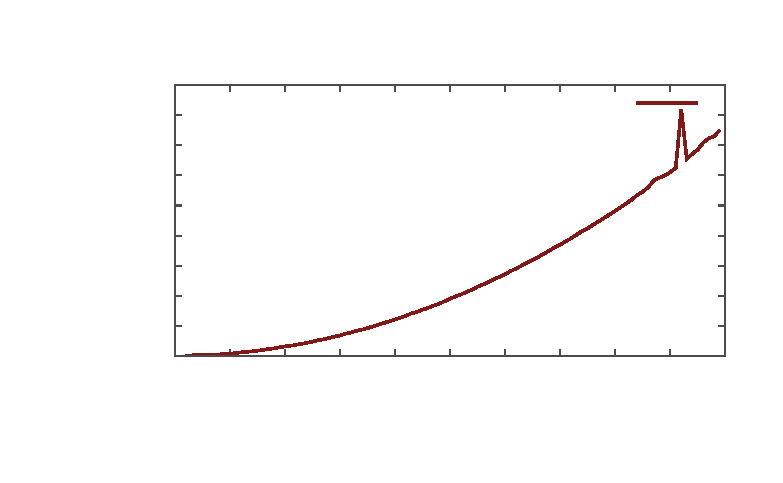
\includegraphics{graficos/mezcla-vectores-clasico}}%
    \gplfronttext
  \end{picture}%
\endgroup

\end{center}

\subsection*{Eficiencia \textit{híbrida}}

\section*{Algoritmo clásico v2}

Como otra alternativa al algoritmo clásico, hemos planteado una segunda version donde se crea un vector de tamaño $k$ que guarda las posiciones máximas de cada vector. \\

Inicializamos el vector de índices con $n - 1$ (ya que están todos los vectores ordenados) y pasamos en cada iteración del bucle cogiendo el índice que corresponda hasta obtener el índice del vector que contiene el máximo valor. Lo añadimos empezando por el final del vector y decrementamos el índice en el vector de índices. \\

El código del programa completo se puede encontrar en la carpeta \textit{src}.

\lstinputlisting[language=C++, linerange={12-43}]{./src/mezcla-vectores-clasico-v2.cpp}

\subsection*{Eficiencia teorica}

\subsection*{Eficiencia empírica}

En el gráfico que se muestra a continuación se muestran los resultados de la
ejecución del algoritmo \textit{clásico} con vectores de 10 elementos.

\begin{center}
	% GNUPLOT: LaTeX picture with Postscript
\begingroup
  \makeatletter
  \providecommand\color[2][]{%
    \GenericError{(gnuplot) \space\space\space\@spaces}{%
      Package color not loaded in conjunction with
      terminal option `colourtext'%
    }{See the gnuplot documentation for explanation.%
    }{Either use 'blacktext' in gnuplot or load the package
      color.sty in LaTeX.}%
    \renewcommand\color[2][]{}%
  }%
  \providecommand\includegraphics[2][]{%
    \GenericError{(gnuplot) \space\space\space\@spaces}{%
      Package graphicx or graphics not loaded%
    }{See the gnuplot documentation for explanation.%
    }{The gnuplot epslatex terminal needs graphicx.sty or graphics.sty.}%
    \renewcommand\includegraphics[2][]{}%
  }%
  \providecommand\rotatebox[2]{#2}%
  \@ifundefined{ifGPcolor}{%
    \newif\ifGPcolor
    \GPcolortrue
  }{}%
  \@ifundefined{ifGPblacktext}{%
    \newif\ifGPblacktext
    \GPblacktextfalse
  }{}%
  % define a \g@addto@macro without @ in the name:
  \let\gplgaddtomacro\g@addto@macro
  % define empty templates for all commands taking text:
  \gdef\gplbacktext{}%
  \gdef\gplfronttext{}%
  \makeatother
  \ifGPblacktext
    % no textcolor at all
    \def\colorrgb#1{}%
    \def\colorgray#1{}%
  \else
    % gray or color?
    \ifGPcolor
      \def\colorrgb#1{\color[rgb]{#1}}%
      \def\colorgray#1{\color[gray]{#1}}%
      \expandafter\def\csname LTw\endcsname{\color{white}}%
      \expandafter\def\csname LTb\endcsname{\color{black}}%
      \expandafter\def\csname LTa\endcsname{\color{black}}%
      \expandafter\def\csname LT0\endcsname{\color[rgb]{1,0,0}}%
      \expandafter\def\csname LT1\endcsname{\color[rgb]{0,1,0}}%
      \expandafter\def\csname LT2\endcsname{\color[rgb]{0,0,1}}%
      \expandafter\def\csname LT3\endcsname{\color[rgb]{1,0,1}}%
      \expandafter\def\csname LT4\endcsname{\color[rgb]{0,1,1}}%
      \expandafter\def\csname LT5\endcsname{\color[rgb]{1,1,0}}%
      \expandafter\def\csname LT6\endcsname{\color[rgb]{0,0,0}}%
      \expandafter\def\csname LT7\endcsname{\color[rgb]{1,0.3,0}}%
      \expandafter\def\csname LT8\endcsname{\color[rgb]{0.5,0.5,0.5}}%
    \else
      % gray
      \def\colorrgb#1{\color{black}}%
      \def\colorgray#1{\color[gray]{#1}}%
      \expandafter\def\csname LTw\endcsname{\color{white}}%
      \expandafter\def\csname LTb\endcsname{\color{black}}%
      \expandafter\def\csname LTa\endcsname{\color{black}}%
      \expandafter\def\csname LT0\endcsname{\color{black}}%
      \expandafter\def\csname LT1\endcsname{\color{black}}%
      \expandafter\def\csname LT2\endcsname{\color{black}}%
      \expandafter\def\csname LT3\endcsname{\color{black}}%
      \expandafter\def\csname LT4\endcsname{\color{black}}%
      \expandafter\def\csname LT5\endcsname{\color{black}}%
      \expandafter\def\csname LT6\endcsname{\color{black}}%
      \expandafter\def\csname LT7\endcsname{\color{black}}%
      \expandafter\def\csname LT8\endcsname{\color{black}}%
    \fi
  \fi
  \setlength{\unitlength}{0.0500bp}%
  \begin{picture}(7200.00,4320.00)%
    \gplgaddtomacro\gplbacktext{%
      \colorrgb{0.30,0.30,0.30}%
      \put(1474,1324){\makebox(0,0)[r]{\strut{}$\textcolor{text}{0}$}}%
      \colorrgb{0.30,0.30,0.30}%
      \put(1474,1583){\makebox(0,0)[r]{\strut{}$\textcolor{text}{0.1}$}}%
      \colorrgb{0.30,0.30,0.30}%
      \put(1474,1843){\makebox(0,0)[r]{\strut{}$\textcolor{text}{0.2}$}}%
      \colorrgb{0.30,0.30,0.30}%
      \put(1474,2102){\makebox(0,0)[r]{\strut{}$\textcolor{text}{0.3}$}}%
      \colorrgb{0.30,0.30,0.30}%
      \put(1474,2362){\makebox(0,0)[r]{\strut{}$\textcolor{text}{0.4}$}}%
      \colorrgb{0.30,0.30,0.30}%
      \put(1474,2621){\makebox(0,0)[r]{\strut{}$\textcolor{text}{0.5}$}}%
      \colorrgb{0.30,0.30,0.30}%
      \put(1474,2881){\makebox(0,0)[r]{\strut{}$\textcolor{text}{0.6}$}}%
      \colorrgb{0.30,0.30,0.30}%
      \put(1474,3140){\makebox(0,0)[r]{\strut{}$\textcolor{text}{0.7}$}}%
      \colorrgb{0.30,0.30,0.30}%
      \put(1474,3400){\makebox(0,0)[r]{\strut{}$\textcolor{text}{0.8}$}}%
      \colorrgb{0.30,0.30,0.30}%
      \put(1474,3659){\makebox(0,0)[r]{\strut{}$\textcolor{text}{0.9}$}}%
      \colorrgb{0.30,0.30,0.30}%
      \put(1606,1192){\rotatebox{45}{\makebox(0,0)[r]{\strut{}$\textcolor{text}{0}$}}}%
      \colorrgb{0.30,0.30,0.30}%
      \put(2126,1192){\rotatebox{45}{\makebox(0,0)[r]{\strut{}$\textcolor{text}{500}$}}}%
      \colorrgb{0.30,0.30,0.30}%
      \put(2645,1192){\rotatebox{45}{\makebox(0,0)[r]{\strut{}$\textcolor{text}{1000}$}}}%
      \colorrgb{0.30,0.30,0.30}%
      \put(3165,1192){\rotatebox{45}{\makebox(0,0)[r]{\strut{}$\textcolor{text}{1500}$}}}%
      \colorrgb{0.30,0.30,0.30}%
      \put(3685,1192){\rotatebox{45}{\makebox(0,0)[r]{\strut{}$\textcolor{text}{2000}$}}}%
      \colorrgb{0.30,0.30,0.30}%
      \put(4205,1192){\rotatebox{45}{\makebox(0,0)[r]{\strut{}$\textcolor{text}{2500}$}}}%
      \colorrgb{0.30,0.30,0.30}%
      \put(4724,1192){\rotatebox{45}{\makebox(0,0)[r]{\strut{}$\textcolor{text}{3000}$}}}%
      \colorrgb{0.30,0.30,0.30}%
      \put(5244,1192){\rotatebox{45}{\makebox(0,0)[r]{\strut{}$\textcolor{text}{3500}$}}}%
      \colorrgb{0.30,0.30,0.30}%
      \put(5764,1192){\rotatebox{45}{\makebox(0,0)[r]{\strut{}$\textcolor{text}{4000}$}}}%
      \colorrgb{0.30,0.30,0.30}%
      \put(6283,1192){\rotatebox{45}{\makebox(0,0)[r]{\strut{}$\textcolor{text}{4500}$}}}%
      \colorrgb{0.30,0.30,0.30}%
      \put(6803,1192){\rotatebox{45}{\makebox(0,0)[r]{\strut{}$\textcolor{text}{5000}$}}}%
      \csname LTb\endcsname%
      \put(176,2491){\rotatebox{-270}{\makebox(0,0){\strut{}Tiempo de ejecución (s)}}}%
      \put(4204,154){\makebox(0,0){\strut{}Número de vectores (k)}}%
      \put(4204,3989){\makebox(0,0){\strut{}Eficiencia empírica mezcla-vectores-clasico-v2}}%
    }%
    \gplgaddtomacro\gplfronttext{%
      \csname LTb\endcsname%
      \put(5816,3486){\makebox(0,0)[r]{\strut{}Algoritmo clásico n = 10}}%
    }%
    \gplbacktext
    \put(0,0){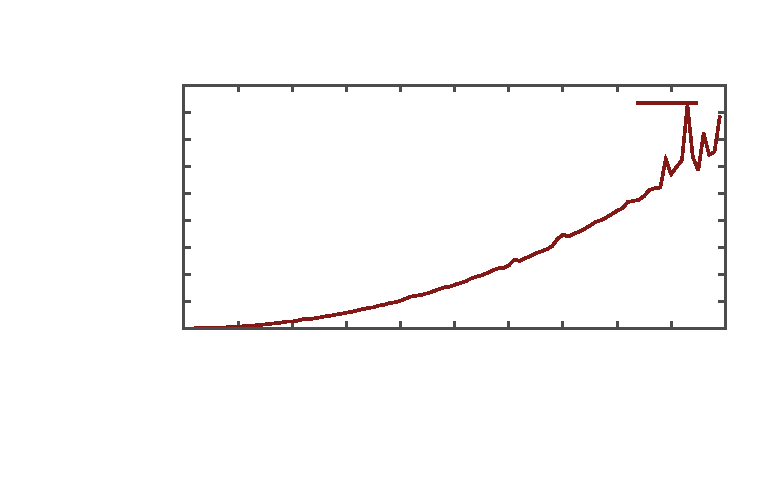
\includegraphics{graficos/mezcla-vectores-clasico-v2}}%
    \gplfronttext
  \end{picture}%
\endgroup

\end{center}

\section*{Algoritmo \textit{divide y vencerás} con vectores dinámicos}


A continuación se proporciona el código de la función \texttt{mezclaDV},
que utiliza un algoritmo divide y vencerás (con vectores dinámicos) para mezclar $k$ vectores en uno solo. El
código del programa completo se puede encontrar en la carpeta \textit{src}.

\lstinputlisting[language=C++, linerange={83-104}]{./src/mezcla-vectores-DyV.cpp}

\subsection*{Eficiencia teórica}

\subsection*{Eficiencia empírica}

En el gráfico que se muestra a continuación se muestran los resultados de la
ejecución del algoritmo \textit{divide y vencerás} con vectores dinámicos de 10 elementos.

\begin{center}
	% GNUPLOT: LaTeX picture with Postscript
\begingroup
  \makeatletter
  \providecommand\color[2][]{%
    \GenericError{(gnuplot) \space\space\space\@spaces}{%
      Package color not loaded in conjunction with
      terminal option `colourtext'%
    }{See the gnuplot documentation for explanation.%
    }{Either use 'blacktext' in gnuplot or load the package
      color.sty in LaTeX.}%
    \renewcommand\color[2][]{}%
  }%
  \providecommand\includegraphics[2][]{%
    \GenericError{(gnuplot) \space\space\space\@spaces}{%
      Package graphicx or graphics not loaded%
    }{See the gnuplot documentation for explanation.%
    }{The gnuplot epslatex terminal needs graphicx.sty or graphics.sty.}%
    \renewcommand\includegraphics[2][]{}%
  }%
  \providecommand\rotatebox[2]{#2}%
  \@ifundefined{ifGPcolor}{%
    \newif\ifGPcolor
    \GPcolortrue
  }{}%
  \@ifundefined{ifGPblacktext}{%
    \newif\ifGPblacktext
    \GPblacktextfalse
  }{}%
  % define a \g@addto@macro without @ in the name:
  \let\gplgaddtomacro\g@addto@macro
  % define empty templates for all commands taking text:
  \gdef\gplbacktext{}%
  \gdef\gplfronttext{}%
  \makeatother
  \ifGPblacktext
    % no textcolor at all
    \def\colorrgb#1{}%
    \def\colorgray#1{}%
  \else
    % gray or color?
    \ifGPcolor
      \def\colorrgb#1{\color[rgb]{#1}}%
      \def\colorgray#1{\color[gray]{#1}}%
      \expandafter\def\csname LTw\endcsname{\color{white}}%
      \expandafter\def\csname LTb\endcsname{\color{black}}%
      \expandafter\def\csname LTa\endcsname{\color{black}}%
      \expandafter\def\csname LT0\endcsname{\color[rgb]{1,0,0}}%
      \expandafter\def\csname LT1\endcsname{\color[rgb]{0,1,0}}%
      \expandafter\def\csname LT2\endcsname{\color[rgb]{0,0,1}}%
      \expandafter\def\csname LT3\endcsname{\color[rgb]{1,0,1}}%
      \expandafter\def\csname LT4\endcsname{\color[rgb]{0,1,1}}%
      \expandafter\def\csname LT5\endcsname{\color[rgb]{1,1,0}}%
      \expandafter\def\csname LT6\endcsname{\color[rgb]{0,0,0}}%
      \expandafter\def\csname LT7\endcsname{\color[rgb]{1,0.3,0}}%
      \expandafter\def\csname LT8\endcsname{\color[rgb]{0.5,0.5,0.5}}%
    \else
      % gray
      \def\colorrgb#1{\color{black}}%
      \def\colorgray#1{\color[gray]{#1}}%
      \expandafter\def\csname LTw\endcsname{\color{white}}%
      \expandafter\def\csname LTb\endcsname{\color{black}}%
      \expandafter\def\csname LTa\endcsname{\color{black}}%
      \expandafter\def\csname LT0\endcsname{\color{black}}%
      \expandafter\def\csname LT1\endcsname{\color{black}}%
      \expandafter\def\csname LT2\endcsname{\color{black}}%
      \expandafter\def\csname LT3\endcsname{\color{black}}%
      \expandafter\def\csname LT4\endcsname{\color{black}}%
      \expandafter\def\csname LT5\endcsname{\color{black}}%
      \expandafter\def\csname LT6\endcsname{\color{black}}%
      \expandafter\def\csname LT7\endcsname{\color{black}}%
      \expandafter\def\csname LT8\endcsname{\color{black}}%
    \fi
  \fi
    \setlength{\unitlength}{0.0500bp}%
    \ifx\gptboxheight\undefined%
      \newlength{\gptboxheight}%
      \newlength{\gptboxwidth}%
      \newsavebox{\gptboxtext}%
    \fi%
    \setlength{\fboxrule}{0.5pt}%
    \setlength{\fboxsep}{1pt}%
\begin{picture}(7200.00,4320.00)%
    \gplgaddtomacro\gplbacktext{%
      \colorrgb{0.30,0.30,0.30}%
      \put(1518,1060){\makebox(0,0)[r]{\strut{}$\textcolor{text}{0}$}}%
      \colorrgb{0.30,0.30,0.30}%
      \put(1518,1431){\makebox(0,0)[r]{\strut{}$\textcolor{text}{0.001}$}}%
      \colorrgb{0.30,0.30,0.30}%
      \put(1518,1803){\makebox(0,0)[r]{\strut{}$\textcolor{text}{0.002}$}}%
      \colorrgb{0.30,0.30,0.30}%
      \put(1518,2174){\makebox(0,0)[r]{\strut{}$\textcolor{text}{0.003}$}}%
      \colorrgb{0.30,0.30,0.30}%
      \put(1518,2545){\makebox(0,0)[r]{\strut{}$\textcolor{text}{0.004}$}}%
      \colorrgb{0.30,0.30,0.30}%
      \put(1518,2916){\makebox(0,0)[r]{\strut{}$\textcolor{text}{0.005}$}}%
      \colorrgb{0.30,0.30,0.30}%
      \put(1518,3288){\makebox(0,0)[r]{\strut{}$\textcolor{text}{0.006}$}}%
      \colorrgb{0.30,0.30,0.30}%
      \put(1518,3659){\makebox(0,0)[r]{\strut{}$\textcolor{text}{0.007}$}}%
      \colorrgb{0.30,0.30,0.30}%
      \put(1650,928){\rotatebox{45}{\makebox(0,0)[r]{\strut{}$\textcolor{text}{0}$}}}%
      \colorrgb{0.30,0.30,0.30}%
      \put(2165,928){\rotatebox{45}{\makebox(0,0)[r]{\strut{}$\textcolor{text}{500}$}}}%
      \colorrgb{0.30,0.30,0.30}%
      \put(2681,928){\rotatebox{45}{\makebox(0,0)[r]{\strut{}$\textcolor{text}{1000}$}}}%
      \colorrgb{0.30,0.30,0.30}%
      \put(3196,928){\rotatebox{45}{\makebox(0,0)[r]{\strut{}$\textcolor{text}{1500}$}}}%
      \colorrgb{0.30,0.30,0.30}%
      \put(3711,928){\rotatebox{45}{\makebox(0,0)[r]{\strut{}$\textcolor{text}{2000}$}}}%
      \colorrgb{0.30,0.30,0.30}%
      \put(4227,928){\rotatebox{45}{\makebox(0,0)[r]{\strut{}$\textcolor{text}{2500}$}}}%
      \colorrgb{0.30,0.30,0.30}%
      \put(4742,928){\rotatebox{45}{\makebox(0,0)[r]{\strut{}$\textcolor{text}{3000}$}}}%
      \colorrgb{0.30,0.30,0.30}%
      \put(5257,928){\rotatebox{45}{\makebox(0,0)[r]{\strut{}$\textcolor{text}{3500}$}}}%
      \colorrgb{0.30,0.30,0.30}%
      \put(5772,928){\rotatebox{45}{\makebox(0,0)[r]{\strut{}$\textcolor{text}{4000}$}}}%
      \colorrgb{0.30,0.30,0.30}%
      \put(6288,928){\rotatebox{45}{\makebox(0,0)[r]{\strut{}$\textcolor{text}{4500}$}}}%
      \colorrgb{0.30,0.30,0.30}%
      \put(6803,928){\rotatebox{45}{\makebox(0,0)[r]{\strut{}$\textcolor{text}{5000}$}}}%
    }%
    \gplgaddtomacro\gplfronttext{%
      \colorrgb{0.30,0.30,0.30}%
      \put(220,2359){\rotatebox{-270}{\makebox(0,0){\strut{}Tiempo de ejecución (s)}}}%
      \colorrgb{0.30,0.30,0.30}%
      \put(4226,220){\makebox(0,0){\strut{}Número de vectores (k)}}%
      \colorrgb{0.30,0.30,0.30}%
      \put(4226,3989){\makebox(0,0){\strut{}Eficiencia empírica mezcla-vectores-DyV}}%
      \csname LTb\endcsname%
      \put(5816,3486){\makebox(0,0)[r]{\strut{}Algoritmo divide y vencerás n = 10}}%
    }%
    \gplbacktext
    \put(0,0){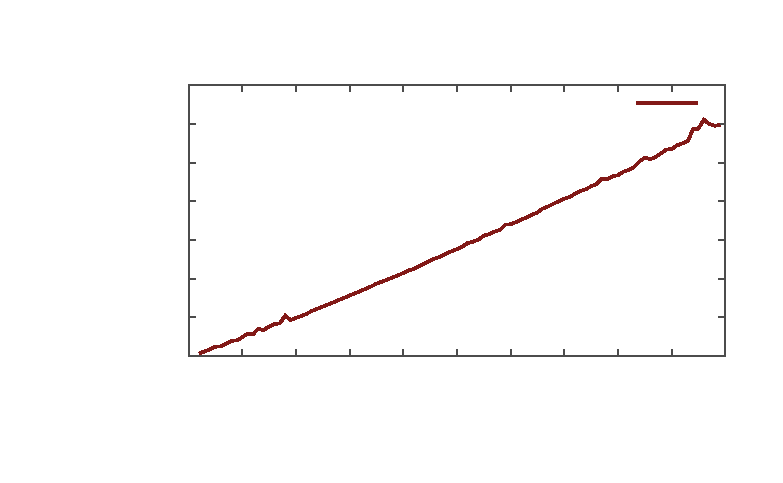
\includegraphics{graficos/mezcla-vectores-DyV}}%
    \gplfronttext
  \end{picture}%
\endgroup

\end{center}

\subsection*{Eficiencia \textit{híbrida}}

\section*{Algoritmo \textit{divide y vencerás} con vectores de la STL}


A continuación se proporciona el código de la función \texttt{mezclaDV},
que utiliza un algoritmo divide y vencerás (con vectores de la STL) para mezclar $k$ vectores en uno solo. El
código del programa completo se puede encontrar en la carpeta \textit{src}.

\lstinputlisting[language=C++, linerange={75-96}]{./src/mezcla-vectores-DyV-STL.cpp}

\subsection*{Eficiencia teórica}

\subsection*{Eficiencia empírica}

En el gráfico que se muestra a continuación se muestran los resultados de la
ejecución del algoritmo \textit{divide y vencerás} con vectores
\texttt{std::vector} de 10 elementos.

\begin{center}
	% GNUPLOT: LaTeX picture with Postscript
\begingroup
  \makeatletter
  \providecommand\color[2][]{%
    \GenericError{(gnuplot) \space\space\space\@spaces}{%
      Package color not loaded in conjunction with
      terminal option `colourtext'%
    }{See the gnuplot documentation for explanation.%
    }{Either use 'blacktext' in gnuplot or load the package
      color.sty in LaTeX.}%
    \renewcommand\color[2][]{}%
  }%
  \providecommand\includegraphics[2][]{%
    \GenericError{(gnuplot) \space\space\space\@spaces}{%
      Package graphicx or graphics not loaded%
    }{See the gnuplot documentation for explanation.%
    }{The gnuplot epslatex terminal needs graphicx.sty or graphics.sty.}%
    \renewcommand\includegraphics[2][]{}%
  }%
  \providecommand\rotatebox[2]{#2}%
  \@ifundefined{ifGPcolor}{%
    \newif\ifGPcolor
    \GPcolortrue
  }{}%
  \@ifundefined{ifGPblacktext}{%
    \newif\ifGPblacktext
    \GPblacktextfalse
  }{}%
  % define a \g@addto@macro without @ in the name:
  \let\gplgaddtomacro\g@addto@macro
  % define empty templates for all commands taking text:
  \gdef\gplbacktext{}%
  \gdef\gplfronttext{}%
  \makeatother
  \ifGPblacktext
    % no textcolor at all
    \def\colorrgb#1{}%
    \def\colorgray#1{}%
  \else
    % gray or color?
    \ifGPcolor
      \def\colorrgb#1{\color[rgb]{#1}}%
      \def\colorgray#1{\color[gray]{#1}}%
      \expandafter\def\csname LTw\endcsname{\color{white}}%
      \expandafter\def\csname LTb\endcsname{\color{black}}%
      \expandafter\def\csname LTa\endcsname{\color{black}}%
      \expandafter\def\csname LT0\endcsname{\color[rgb]{1,0,0}}%
      \expandafter\def\csname LT1\endcsname{\color[rgb]{0,1,0}}%
      \expandafter\def\csname LT2\endcsname{\color[rgb]{0,0,1}}%
      \expandafter\def\csname LT3\endcsname{\color[rgb]{1,0,1}}%
      \expandafter\def\csname LT4\endcsname{\color[rgb]{0,1,1}}%
      \expandafter\def\csname LT5\endcsname{\color[rgb]{1,1,0}}%
      \expandafter\def\csname LT6\endcsname{\color[rgb]{0,0,0}}%
      \expandafter\def\csname LT7\endcsname{\color[rgb]{1,0.3,0}}%
      \expandafter\def\csname LT8\endcsname{\color[rgb]{0.5,0.5,0.5}}%
    \else
      % gray
      \def\colorrgb#1{\color{black}}%
      \def\colorgray#1{\color[gray]{#1}}%
      \expandafter\def\csname LTw\endcsname{\color{white}}%
      \expandafter\def\csname LTb\endcsname{\color{black}}%
      \expandafter\def\csname LTa\endcsname{\color{black}}%
      \expandafter\def\csname LT0\endcsname{\color{black}}%
      \expandafter\def\csname LT1\endcsname{\color{black}}%
      \expandafter\def\csname LT2\endcsname{\color{black}}%
      \expandafter\def\csname LT3\endcsname{\color{black}}%
      \expandafter\def\csname LT4\endcsname{\color{black}}%
      \expandafter\def\csname LT5\endcsname{\color{black}}%
      \expandafter\def\csname LT6\endcsname{\color{black}}%
      \expandafter\def\csname LT7\endcsname{\color{black}}%
      \expandafter\def\csname LT8\endcsname{\color{black}}%
    \fi
  \fi
    \setlength{\unitlength}{0.0500bp}%
    \ifx\gptboxheight\undefined%
      \newlength{\gptboxheight}%
      \newlength{\gptboxwidth}%
      \newsavebox{\gptboxtext}%
    \fi%
    \setlength{\fboxrule}{0.5pt}%
    \setlength{\fboxsep}{1pt}%
\begin{picture}(7200.00,4320.00)%
    \gplgaddtomacro\gplbacktext{%
      \colorrgb{0.30,0.30,0.30}%
      \put(1518,1060){\makebox(0,0)[r]{\strut{}$\textcolor{text}{0}$}}%
      \colorrgb{0.30,0.30,0.30}%
      \put(1518,1431){\makebox(0,0)[r]{\strut{}$\textcolor{text}{0.005}$}}%
      \colorrgb{0.30,0.30,0.30}%
      \put(1518,1803){\makebox(0,0)[r]{\strut{}$\textcolor{text}{0.01}$}}%
      \colorrgb{0.30,0.30,0.30}%
      \put(1518,2174){\makebox(0,0)[r]{\strut{}$\textcolor{text}{0.015}$}}%
      \colorrgb{0.30,0.30,0.30}%
      \put(1518,2545){\makebox(0,0)[r]{\strut{}$\textcolor{text}{0.02}$}}%
      \colorrgb{0.30,0.30,0.30}%
      \put(1518,2916){\makebox(0,0)[r]{\strut{}$\textcolor{text}{0.025}$}}%
      \colorrgb{0.30,0.30,0.30}%
      \put(1518,3288){\makebox(0,0)[r]{\strut{}$\textcolor{text}{0.03}$}}%
      \colorrgb{0.30,0.30,0.30}%
      \put(1518,3659){\makebox(0,0)[r]{\strut{}$\textcolor{text}{0.035}$}}%
      \colorrgb{0.30,0.30,0.30}%
      \put(1650,928){\rotatebox{45}{\makebox(0,0)[r]{\strut{}$\textcolor{text}{0}$}}}%
      \colorrgb{0.30,0.30,0.30}%
      \put(2165,928){\rotatebox{45}{\makebox(0,0)[r]{\strut{}$\textcolor{text}{500}$}}}%
      \colorrgb{0.30,0.30,0.30}%
      \put(2681,928){\rotatebox{45}{\makebox(0,0)[r]{\strut{}$\textcolor{text}{1000}$}}}%
      \colorrgb{0.30,0.30,0.30}%
      \put(3196,928){\rotatebox{45}{\makebox(0,0)[r]{\strut{}$\textcolor{text}{1500}$}}}%
      \colorrgb{0.30,0.30,0.30}%
      \put(3711,928){\rotatebox{45}{\makebox(0,0)[r]{\strut{}$\textcolor{text}{2000}$}}}%
      \colorrgb{0.30,0.30,0.30}%
      \put(4227,928){\rotatebox{45}{\makebox(0,0)[r]{\strut{}$\textcolor{text}{2500}$}}}%
      \colorrgb{0.30,0.30,0.30}%
      \put(4742,928){\rotatebox{45}{\makebox(0,0)[r]{\strut{}$\textcolor{text}{3000}$}}}%
      \colorrgb{0.30,0.30,0.30}%
      \put(5257,928){\rotatebox{45}{\makebox(0,0)[r]{\strut{}$\textcolor{text}{3500}$}}}%
      \colorrgb{0.30,0.30,0.30}%
      \put(5772,928){\rotatebox{45}{\makebox(0,0)[r]{\strut{}$\textcolor{text}{4000}$}}}%
      \colorrgb{0.30,0.30,0.30}%
      \put(6288,928){\rotatebox{45}{\makebox(0,0)[r]{\strut{}$\textcolor{text}{4500}$}}}%
      \colorrgb{0.30,0.30,0.30}%
      \put(6803,928){\rotatebox{45}{\makebox(0,0)[r]{\strut{}$\textcolor{text}{5000}$}}}%
    }%
    \gplgaddtomacro\gplfronttext{%
      \colorrgb{0.30,0.30,0.30}%
      \put(220,2359){\rotatebox{-270}{\makebox(0,0){\strut{}Tiempo de ejecución (s)}}}%
      \colorrgb{0.30,0.30,0.30}%
      \put(4226,220){\makebox(0,0){\strut{}Número de vectores (k)}}%
      \colorrgb{0.30,0.30,0.30}%
      \put(4226,3989){\makebox(0,0){\strut{}Eficiencia empírica mezcla-vectores-DyV-STL}}%
      \csname LTb\endcsname%
      \put(5816,3486){\makebox(0,0)[r]{\strut{}Algoritmo divide y vencerás n = 10}}%
    }%
    \gplbacktext
    \put(0,0){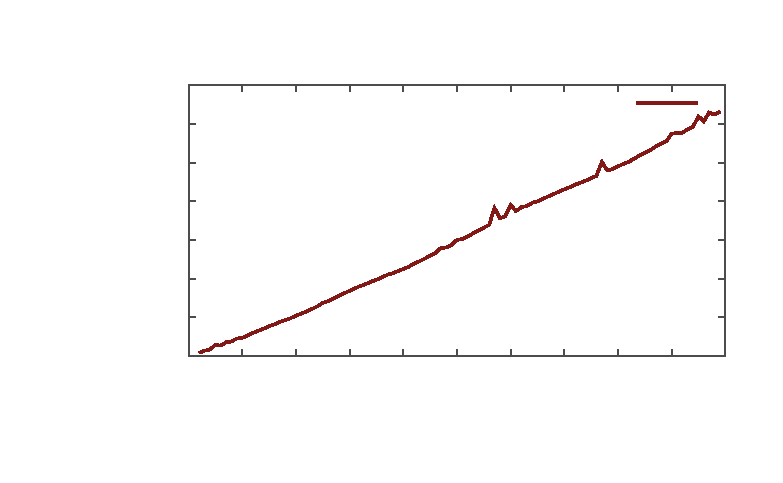
\includegraphics{graficos/mezcla-vectores-DyV-STL}}%
    \gplfronttext
  \end{picture}%
\endgroup

\end{center}

\subsection*{Eficiencia \textit{híbrida}}

\section*{Comparación de la eficiencia}

En el siguiente gráfico se puede observar de forma visual qué algoritmo es más
eficiente. Como es de esperar, el algoritmo clásico es el más lento de
todos. Algo más curioso quizás es que el algoritmo que utiliza vectores
\textit{dinámicos} es más rápido que el que usa la clase \texttt{vector} de la STL.

\begin{center}
	% GNUPLOT: LaTeX picture with Postscript
\begingroup
  \makeatletter
  \providecommand\color[2][]{%
    \GenericError{(gnuplot) \space\space\space\@spaces}{%
      Package color not loaded in conjunction with
      terminal option `colourtext'%
    }{See the gnuplot documentation for explanation.%
    }{Either use 'blacktext' in gnuplot or load the package
      color.sty in LaTeX.}%
    \renewcommand\color[2][]{}%
  }%
  \providecommand\includegraphics[2][]{%
    \GenericError{(gnuplot) \space\space\space\@spaces}{%
      Package graphicx or graphics not loaded%
    }{See the gnuplot documentation for explanation.%
    }{The gnuplot epslatex terminal needs graphicx.sty or graphics.sty.}%
    \renewcommand\includegraphics[2][]{}%
  }%
  \providecommand\rotatebox[2]{#2}%
  \@ifundefined{ifGPcolor}{%
    \newif\ifGPcolor
    \GPcolortrue
  }{}%
  \@ifundefined{ifGPblacktext}{%
    \newif\ifGPblacktext
    \GPblacktextfalse
  }{}%
  % define a \g@addto@macro without @ in the name:
  \let\gplgaddtomacro\g@addto@macro
  % define empty templates for all commands taking text:
  \gdef\gplbacktext{}%
  \gdef\gplfronttext{}%
  \makeatother
  \ifGPblacktext
    % no textcolor at all
    \def\colorrgb#1{}%
    \def\colorgray#1{}%
  \else
    % gray or color?
    \ifGPcolor
      \def\colorrgb#1{\color[rgb]{#1}}%
      \def\colorgray#1{\color[gray]{#1}}%
      \expandafter\def\csname LTw\endcsname{\color{white}}%
      \expandafter\def\csname LTb\endcsname{\color{black}}%
      \expandafter\def\csname LTa\endcsname{\color{black}}%
      \expandafter\def\csname LT0\endcsname{\color[rgb]{1,0,0}}%
      \expandafter\def\csname LT1\endcsname{\color[rgb]{0,1,0}}%
      \expandafter\def\csname LT2\endcsname{\color[rgb]{0,0,1}}%
      \expandafter\def\csname LT3\endcsname{\color[rgb]{1,0,1}}%
      \expandafter\def\csname LT4\endcsname{\color[rgb]{0,1,1}}%
      \expandafter\def\csname LT5\endcsname{\color[rgb]{1,1,0}}%
      \expandafter\def\csname LT6\endcsname{\color[rgb]{0,0,0}}%
      \expandafter\def\csname LT7\endcsname{\color[rgb]{1,0.3,0}}%
      \expandafter\def\csname LT8\endcsname{\color[rgb]{0.5,0.5,0.5}}%
    \else
      % gray
      \def\colorrgb#1{\color{black}}%
      \def\colorgray#1{\color[gray]{#1}}%
      \expandafter\def\csname LTw\endcsname{\color{white}}%
      \expandafter\def\csname LTb\endcsname{\color{black}}%
      \expandafter\def\csname LTa\endcsname{\color{black}}%
      \expandafter\def\csname LT0\endcsname{\color{black}}%
      \expandafter\def\csname LT1\endcsname{\color{black}}%
      \expandafter\def\csname LT2\endcsname{\color{black}}%
      \expandafter\def\csname LT3\endcsname{\color{black}}%
      \expandafter\def\csname LT4\endcsname{\color{black}}%
      \expandafter\def\csname LT5\endcsname{\color{black}}%
      \expandafter\def\csname LT6\endcsname{\color{black}}%
      \expandafter\def\csname LT7\endcsname{\color{black}}%
      \expandafter\def\csname LT8\endcsname{\color{black}}%
    \fi
  \fi
    \setlength{\unitlength}{0.0500bp}%
    \ifx\gptboxheight\undefined%
      \newlength{\gptboxheight}%
      \newlength{\gptboxwidth}%
      \newsavebox{\gptboxtext}%
    \fi%
    \setlength{\fboxrule}{0.5pt}%
    \setlength{\fboxsep}{1pt}%
\begin{picture}(7200.00,4320.00)%
    \gplgaddtomacro\gplbacktext{%
      \colorrgb{0.30,0.30,0.30}%
      \put(1650,1060){\makebox(0,0)[r]{\strut{}$\textcolor{text}{1e-05}$}}%
      \colorrgb{0.30,0.30,0.30}%
      \put(1650,1580){\makebox(0,0)[r]{\strut{}$\textcolor{text}{0.0001}$}}%
      \colorrgb{0.30,0.30,0.30}%
      \put(1650,2100){\makebox(0,0)[r]{\strut{}$\textcolor{text}{0.001}$}}%
      \colorrgb{0.30,0.30,0.30}%
      \put(1650,2619){\makebox(0,0)[r]{\strut{}$\textcolor{text}{0.01}$}}%
      \colorrgb{0.30,0.30,0.30}%
      \put(1650,3139){\makebox(0,0)[r]{\strut{}$\textcolor{text}{0.1}$}}%
      \colorrgb{0.30,0.30,0.30}%
      \put(1650,3659){\makebox(0,0)[r]{\strut{}$\textcolor{text}{1}$}}%
      \colorrgb{0.30,0.30,0.30}%
      \put(1782,928){\rotatebox{45}{\makebox(0,0)[r]{\strut{}$\textcolor{text}{0}$}}}%
      \colorrgb{0.30,0.30,0.30}%
      \put(2093,928){\rotatebox{45}{\makebox(0,0)[r]{\strut{}$\textcolor{text}{500}$}}}%
      \colorrgb{0.30,0.30,0.30}%
      \put(2404,928){\rotatebox{45}{\makebox(0,0)[r]{\strut{}$\textcolor{text}{1000}$}}}%
      \colorrgb{0.30,0.30,0.30}%
      \put(2715,928){\rotatebox{45}{\makebox(0,0)[r]{\strut{}$\textcolor{text}{1500}$}}}%
      \colorrgb{0.30,0.30,0.30}%
      \put(3026,928){\rotatebox{45}{\makebox(0,0)[r]{\strut{}$\textcolor{text}{2000}$}}}%
      \colorrgb{0.30,0.30,0.30}%
      \put(3337,928){\rotatebox{45}{\makebox(0,0)[r]{\strut{}$\textcolor{text}{2500}$}}}%
      \colorrgb{0.30,0.30,0.30}%
      \put(3648,928){\rotatebox{45}{\makebox(0,0)[r]{\strut{}$\textcolor{text}{3000}$}}}%
      \colorrgb{0.30,0.30,0.30}%
      \put(3959,928){\rotatebox{45}{\makebox(0,0)[r]{\strut{}$\textcolor{text}{3500}$}}}%
      \colorrgb{0.30,0.30,0.30}%
      \put(4270,928){\rotatebox{45}{\makebox(0,0)[r]{\strut{}$\textcolor{text}{4000}$}}}%
      \colorrgb{0.30,0.30,0.30}%
      \put(4581,928){\rotatebox{45}{\makebox(0,0)[r]{\strut{}$\textcolor{text}{4500}$}}}%
      \colorrgb{0.30,0.30,0.30}%
      \put(4892,928){\rotatebox{45}{\makebox(0,0)[r]{\strut{}$\textcolor{text}{5000}$}}}%
    }%
    \gplgaddtomacro\gplfronttext{%
      \colorrgb{0.30,0.30,0.30}%
      \put(220,2359){\rotatebox{-270}{\makebox(0,0){\strut{}Tiempo de ejecución (s)}}}%
      \colorrgb{0.30,0.30,0.30}%
      \put(3337,220){\makebox(0,0){\strut{}Número de vectores (k)}}%
      \colorrgb{0.30,0.30,0.30}%
      \put(3337,3989){\makebox(0,0){\strut{}Algoritmos mezcla de k vectores}}%
      \csname LTb\endcsname%
      \put(6212,3549){\makebox(0,0)[r]{\strut{}Clásico}}%
      \csname LTb\endcsname%
      \put(6212,3329){\makebox(0,0)[r]{\strut{}DyV}}%
      \csname LTb\endcsname%
      \put(6212,3109){\makebox(0,0)[r]{\strut{}DyV STL}}%
    }%
    \gplbacktext
    \put(0,0){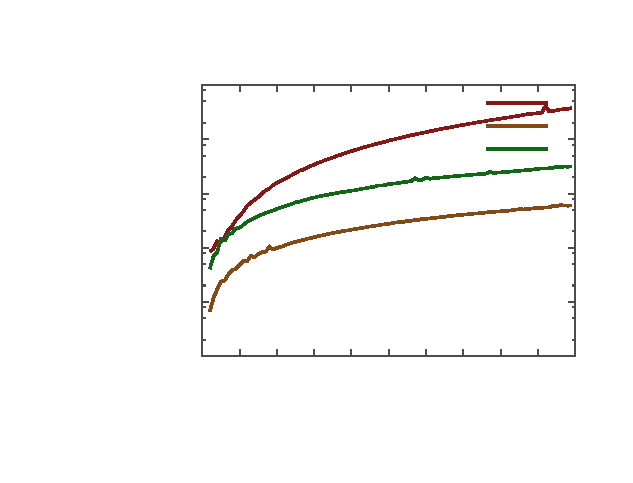
\includegraphics{./graficos/compare}}%
    \gplfronttext
  \end{picture}%
\endgroup

\end{center}




\newpage

\section*{Anexo}
\subsection*{Características de los ordenadores donde se ha ejecutado}

\vspace{0.5em}

\begin{enumerate}
\item Apple MacBook Pro, Intel(R) Core(TM) i5-5257U CPU @ 2.70GHz, 8GB RAM.\\  Compilador: clang-800.0.38 \\
  Sistema operativo: macOS Sierra
\item Dell XPS 13, Intel(R) Core(TM) i5-7200U CPU @ 2.50GHz, 8GB RAM.\\
  Compilador: g++ 6.3.1\\
  Sistema operativo: Arch Linux
\end{enumerate}


\end{document}

